%-------------------------------------------------------
% SLEPc Users Manual
%-------------------------------------------------------
\chapter{\label{cap:back}Background Material}
%-------------------------------------------------------

\section{The Eigenvalue Problem}
\label{sec:eig}

	The eigenvalue problem is a central topic in numerical linear algebra. In the standard formulation, the problem consists in the determination of $\lambda\in\Co$ for which the equation
\begin{equation}Ax=\lambda x\;\;\label{eq:eigstd}\end{equation}
has nontrivial solution, where $A\in\Co^{n\times n}$ and $x \in \Co^n$. The scalar $\lambda$ and the vector $x$ are called eigenvalue and eigenvector, respectively.

	In many applications, the problem is formulated as $Ax=\lambda Bx$, which is known as the generalized eigenvalue problem. Usually, this problem is solved by reformulating it in standard form, as discussed in section \ref{sec:nonstd}.

	Similarity transformations preserve eigenvalues. Two matrices $A$ and $\tilde{A}$ are similar if a non-singular matrix $X$ exists such that $A=X\tilde{A}X^{-1}$. Many methods for eigenvalue problems rely on such transformations in order to reduce the matrix to a canonical form from which it is easier to retrieve eigenpairs. Among these methods are the ones considered to be the fastest and most accurate methods, such as Divide and Conquer, QR Iteration and Jacobi methods. For an up-to-date survey on methods for eigenvalue problems see \citep{Golub:2000:EC2}.

	However, these methods are not appropriate for large sparse matrices because similarity transformations destroy sparsity. Moreover, most applications require only to know a few selected eigenvalues and not the entire spectrum. For these reasons, other methods have become popular for sparse problems. 

\subsection{Basic Methods}

	Methods for sparse eigenproblems obtain the solution from the information generated by the application of the operator to various vectors. That is, the matrix is only used in matrix-vector products. This not only maintains sparsity but allows to solve problems in which matrices are not available explicitly. A catalog of such methods can also be found in \citep{Golub:2000:EC2}. For a more comprehensive description see \citep{Bai:2000:TSA}.

	The most basic method of this kind is the Power Iteration, in which an initial vector is repeatedly premultiplied by the matrix $A$ and conveniently normalized. After a certain number of iterations, this vector converges to the dominant eigenvector, which is the one associated to the eigenvalue with largest module. In many situations, the particular properties of the spectrum can prevent the Power Method from converging. Also, it is usual to require more than just one eigenvalue. For these reasons, more powerful methods are required.

	The Simultaneous Iteration or Subspace Iteration is the generalization of the Power Method. In this method, the matrix is applied to a set of $m$ vectors simultaneously, and orthogonality is enforced explicitly in order to avoid the convergence of all these vectors to the dominant eigenvector.

	In some sense, the power method throws away potentially useful spectral information during the course of the iteration. At the $k$-th iteration, the algorithm overwrites the vector $A^{k-1}x^{(0)}$ with $A^kx^{(0)}$, where $x^{(0)}$ is the initial vector. However, it turns out to be useful to keep the previous vector instead of overwriting it, and by extension to keep the whole set of previous vectors. The subspace
\begin{equation}
\K_m(A,v)\equiv\mathrm{span}\left\{v,Av,A^2v,\ldots,A^{m-1}v\right\}\;\;,
\label{eq:krylov}
\end{equation}
is called the $m$-th Krylov subspace corresponding to $A$ and $v$. Methods which use linear combinations of vectors in this space to extract spectral information are called Krylov subspace methods. The most basic methods of this kind are the Lanczos, non-symmetric Lanczos and Arnoldi algorithms.

	The basic idea of these methods is to construct approximate eigenvectors in the Krylov subspace $\K_m(A,v)$. A Ritz pair is any pair $(\lambda_i,x_i)$ that satisfies the Galerkin condition,
\begin{equation}
\label{eq:galerkin}
(Ax_i-\lambda_i x_i,\,v)=0\;\;,\;\;\;\;\forall v\in\K_m(A,v)\;\;.
\end{equation}
That is, the Ritz pair satisfies the eigenvalue-eigenvector relationship in the projection onto a smaller space. If the component orthogonal to this space is sufficiently small then the Ritz pair is a good approximation to an eigenpair of $A$. The procedure for constructing approximate eigenpairs in this way is called Rayleigh-Ritz projection.

	The following is the Lanczos method:
\begin{tabbing}
xxxx\=xxx\=xxxxxxxxxxxxxxx\=\kill
\> Select an initial vector $v_1$ of norm 1\\
\> Initialize $\beta_1=0$, $v_0=0$\\
\> For $j=1,2,\ldots,k$\\
\> \> $w_j=Av_j-\beta_j v_{j-1}$ \\
\> \> $\alpha_j=v_j^Hw_j$ \\
\> \> $w_j=w_j-\alpha_j v_j$ \\
\> \> $\beta_{j+1}=\|w_j\|_2$ \\
\> \> $v_{j+1}=w_j/\beta_{j+1}$ \\
\> end
\end{tabbing}
This algorithm builds an orthonormal basis $V_k=[v_1,\ldots,v_k]$ and computes a tridiagonal matrix $T_k$, where $\alpha_j$ and $\beta_j$ form the diagonal and sub-diagonal elements, respectively, so that $T_k=V_k^TAV_k$. Let $(\lambda,y)$ be an eigenpair of $T_k$, i.e., $T_ky=\lambda y$, then $\lambda$ is a Ritz value of $A$ and the corresponding Ritz vector is $x=V_ky$. In practice, the Lanczos vectors $v_j$ may lose orthogonality when the above algorithm is carried out in floating-point arithmetic. Some strategies can be used to avoid this problem, including partial or selective re-orthogonalization and elimination of spurious eigenvalues.

	In order to be able to solve non-symmetric eigenproblems, the non-symmetric Lanczos method uses two bi-orthonormal basis to construct a non-symmetric tridiagonal matrix.

	The Arnoldi method, which is also intended for the non-symmetric case, builds a $k$-step Arnoldi factorization,
\begin{equation}
\label{eq:arn}
AV_k=V_kH_k+f_ke_k^T\;\;,
\end{equation}
where the columns of $V_k$ are orthonormal, $V_k^Hf_k=0$, and $H_k$ is an upper Hessenberg matrix of order $k$. As in the Lanczos method, eigenpairs of $H_k$ can be used for building Ritz pairs. The Arnoldi algorithm can be written as follows.
	\begin{tabbing}
xxxx\=xxx\=xxxxxxxxxxxxxxx\=\kill
\> Select an initial vector $v_1$ of norm 1\\
\> For $j=1,2,\ldots,k$\\
\> \> $h_{ij}=v_j^HAv_i,\;i=1,2,\ldots,j$ \\
\> \> $w_j=Av_j-\sum_{i=1}^j h_{ij}v_i$ \\
\> \> $h_{j+1,j}=\|w_j\|_2\;$.\> If $h_{j+1,j}=0$ Stop \\
\> \> $v_{j+1}=w_j/h_{j+1,j}$ \\
\> end\\
\> $f_k=h_{k+1,k}v_{k+1}$
\end{tabbing}
The above algorithm uses the classical Gram-Schmidt orthogonalization scheme when constructing the basis. Other schemes are usually preferred in order to avoid problems with round-off errors.

\subsection{Convergence}

	The Power Method is used to compute a single eigenvector. A simple modification can be done to find the $k$ dominant eigenvectors: once the eigenpair $(\lambda_1,x_1)$ is computed, a transformation is applied to the matrix $A$ to move $\lambda_1$ to the interior of the spectrum, so that the second largest eigenvalue $\lambda_2$ becomes the dominant eigenvalue of the transformed matrix. This process is repeated until the $k$ dominant eigenvalues have been found. This technique is called {\em deflation\/} and it appears implicitly in many other algorithms.

	In methods such as Subspace Iteration or Lanczos, the convergence rate is different from one eigenpair to another. Sometimes the cost of the algorithm can be reduced by {\em locking\/} eigenvectors once they have already converged to desired accuracy. This technique is another form of deflation.

	Convergence problems can arise in the presence of multiple or clustered eigenvalues. Selecting a sufficiently large number of basis vectors can usually avoid the problem. However, convergence can still be very slow and acceleration techniques must be used. Usually, these techniques consists in computing eigenpairs of a transformed operator and then recovering the solution of the original problem. 

	The aim of these transformations is twofold. On one hand, they allow to obtain eigenvalues other than those lying in the boundary of the spectrum. On the other hand, the eigenvalues of interest are well separated in the transformed spectrum thus leading to fast convergence. Sometimes, the transformation can also be constructed to explicitly damp unwanted eigenvalues.

	The simplest transformation is to use the shifted matrix $A+\sigma I$. Other transforms are shift-and-invert $(A-\sigma I)^{-1}$, Cayley $(A-\sigma I)^{-1}(A+\sigma I)$ and, in general, polynomial $p(A)$ or even rational $p(A)q(A)^{-1}$ transformations. The most commonly used one is the shift-and-invert transformation, which allows to compute the eigenvalues closest to $\sigma$ with very good separation properties. When using this approach, a linear system of equations, $(A-\sigma I)y=x$, must be solved in each iteration of the eigenvalue process.

\subsection{Non-standard Problems}
\label{sec:nonstd}

	Although there are specific methods for the generalized eigenvalue problem, $Ax=\lambda Bx$, it is usually solved by reducing it to standard form. There are several possibilities for doing this. If $B$ is non-singular, the problem can be written as
\begin{equation}
\label{eq:invreg}
B^{-1}Ax=\lambda x\;\;.
\end{equation}
If $B$ is singular or ill-conditioned, the roles of $A$ and $B$ can be reversed. On the other hand, if $B$ is symmetric positive definite then the problem is equivalent to
\begin{equation}
L^{-1}A L^{-T}y=\lambda y\;\;,
\end{equation}
where $y=L^Tx$ and $L$ is lower triangular such that $B=LL^T$. 

	In any case, a system of linear equations must be solved in each iteration of the eigensolver. For this reason, using the shift-and-invert technique does not add extra complexity. In this case, after solving the transformed problem
\begin{equation}
\label{eq:sinvg}
(A-\sigma B)^{-1}Bx=\theta x\;\;,
\end{equation}
the eigenvalues of the original problem can be recovered as $\lambda=\frac{1}{\theta}+\sigma$ while the eigenvectors stay the same. Note that this transformation is valid regardless of the regularity of $B$.

	When using equations (\ref{eq:invreg}) or (\ref{eq:sinvg}) symmetry is lost. In order to be able to use methods such as Lanczos which assume a symmetric operator, Euclidean products and norms must be replaced by B-inner products and B-norms.

	In many applications such as the analysis of damped vibrating systems the eigenproblem to be solved is quadratic,
\begin{equation}(A\lambda^2+B\lambda+C)x=0\;\;.\label{eq:eigcuad}\end{equation}
It is possible to transform this problem to a generalized eigenproblem by increasing the order of the system. For example, let the eigenvector be $v=[\lambda x, x]^T$, then the equivalent system is
\begin{equation}
\label{eq:quad}
\left[\begin{array}{cc}-B & -C\\I & 0\end{array}\right]v=\lambda\left[\begin{array}{cc}\;A\; & 0\\0 & \;I\;\end{array}\right]v\;\;.
\end{equation}
	Other linear algebra problems are very closely related to eigenproblems. One of them is the {\em singular value decomposition\/} (SVD). Let $A$ be a real $m\times n$ matrix, then there exist two orthogonal matrices $U\in\Real^{m\times m}$, $V\in\Real^{n\times n}$ such that
\begin{equation}
\label{eq:svd}
U^T\!A\,V=\mathrm{diag}(\sigma_1,\ldots,\sigma_p)\;\;,
\end{equation}
with $p=\min\{m,n\}$ and $\sigma_1\geq\sigma_2\geq\ldots\geq\sigma_p\geq 0$. The values $\sigma_i$ are called singular values. The relation (\ref{eq:svd}) can be expressed as an eigenproblem in several ways, for example
\begin{equation}
\label{eq:svdata}
A^T\!A\,v_i=\sigma_i^2v_i\;\;,
\end{equation}
or
\begin{equation}
\label{eq:svd2}
\left[\begin{array}{cc}0&A\\A^T&0\end{array}\right]
\left[\begin{array}{c}u_i\\v_i\end{array}\right]=\sigma_i
\left[\begin{array}{c}u_i\\v_i\end{array}\right]\;\;.
\end{equation}

\subsection{State-of-the-art Methods}

	One drawback of the Arnoldi algorithm with respect to Lanczos is the increment of cost and storage as the size of the subspace increases. The solution to this is to restart the Arnoldi reduction when a certain size is reached. The Implicit Restart technique allows to filter away unwanted information from the process. This leads to a reduced subspace with a basis for which the matrix still has a Hessenberg form, so that Arnoldi's process can be continued with a subspace (rather than with a single vector as with more classical restart techniques). This Implicitly Restarted Arnoldi method is the one implemented in \arpack. Another strategy called thick-restarting has been proposed to achieve similar effectiveness while somewhat reducing the complexity.

	Krylov subspace methods are projection methods because they project the original matrix onto a certain subspace. Other projection methods use the same idea but with a different type of subspace. One of these techniques, called Rational Krylov Sequence (RKS), combines a spectral transformation such as shift-and-invert with a modification of the shift in each step. The result is the generation of the so-called rational Krylov subspace
\begin{equation}
\mathrm{span}\left\{v,T_1^{SI}v,\ldots,\left(T_{m-1}^{SI}\cdots T_1^{SI}\right)v\right\}\;\;,
\label{eq:rat-krylov}
\end{equation}
where $T_j^{SI}=(A-\sigma_j B)^{-1}B$. Since the matrix $A-\sigma_j B$ changes at every step, it is not feasible to compute a factorization at the beginning and then reuse the factors to solve the system at each iteration. Iterative linear solvers may be preferred in this case.

	Another approach is Davidson's method which expands the subspace by orthogonalizing $\tilde{v}$ with respect to the previous basis vectors. This vector $\tilde{v}$ is the solution of the linear system of equations $(D\!_A-\theta I)\tilde{v}=r$, where $D\!_A$ is the diagonal of matrix $A$, $r$ is the defect $r=Au-\theta u$, and $(\theta,u)$ is a Ritz pair. This method was enhanced later by introducing a correction $\Delta u$ for $u$ in the subspace orthogonal to $u$. In this case, the linear system to be solved is
\begin{equation}
(I-uu^H)(A-\theta I)(I-uu^H)\Delta u=-r\;\;,
\end{equation}
and the whole process constitutes the Jacobi-Davidson method.

	Finally, the block-oriented analogues of some of the methods described above can be very effective in some situations. An example of this is the ABLE method, a block Lanczos algorithm which adaptively adjusts the block size.

\subsection{Available Software}

	The development of high-quality software for eigenvalue problems starts with the book edited by \cite{Wilkinson:1971:LA} which contained implementations in Algol60 of many algorithms for the solution of linear systems of equations and eigenvalue problems. In the early 1970's, these algorithms gave way to the packages \linpack\ and \eispack, which were written in Fortran. \eispack\ \citep{Smith:1970:MER}, which concentrates on eigenvalue problems, is the first library approaching this kind of problems in a rigorous way. These libraries are the basement of more recent software such as the commercial packages {\sc imsl} and {\sc nag}, or even \matlab. In the 1990's, \linpack\ and \eispack\ were replaced by \lapack\ \citep{Anderson:1992:LUG}, a completely rewritten library which already guarantees reliability, portability and efficiency in a systematic way. It implements block-oriented versions of the algorithms and makes extensive use of the level 3 Basic Linear Algebra Subprograms (\blas). Most of the algorithms for eigenvalue problems included in \lapack\ have their parallel counterpart in \scalapack\ \citep{Blackford:1997:SUG}, today the main source of parallel algorithms for dense linear algebra problems.
	
	Unlike in dense methods, there are few standards for basic sparse operations in the spirit of \blas. This is due to the fact that sparse storage is more complicated, admitting of more variation, and therefore less standardized. For this reason, sparse libraries have an added level of complexity. This holds even more so in the parallel case, where additional indexing information is needed to specify which matrix elements are on which processor.
	
	The first implementations of algorithms for sparse matrices appeared in the journal {\em Transactions on Mathematical Software\/}, for example \lopsi\ \citep{Stewart:1981:ALS} which implements the Subspace Iteration method. This subroutine required a prescribed storage format for the sparse matrix, which is an obvious limitation. 
	
	An alternative way of matrix representation is by means of a user-provided subroutine for the matrix-vector product. Apart from being format-independent this solution allows to solve problems in which the matrix is not available explicitly. The drawback is the restriction to a fixed-prototype subroutine. This is the option used in \srrit\ \citep{Bai:1997:ASF}, which also implements Subspace Iteration, and \arncheb\ \citep{Braconnier:1993:AAS}, which implements the Arnoldi method with explicit restart. A description and comparison of some of these packages can be found in \citep{Lehoucq:1996:ESC}.
	
	A good solution for the matrix representation problem is the well-known reverse communication interface, a technique which allows to implement iterative methods disregarding the implementation details of various operations. Whenever the iterative method subroutine needs the results of one of the operations, it returns control to the user's subroutine that called it. The user's subroutine then invokes the module that performs the operation. The iterative method subroutine is invoked again with the results of the operation. This scheme is very useful when, for example, the method requires not only the product by the matrix but also the product by the transpose. This is the case of \qmrpack\ \citep{Freund:1996:QPQ}, which implements the non-symmetric Lanczos method. 
	
	More recent software packages implement advanced techniques and are prepared for parallel execution. This is the case of \arpack, \blzpack, \planso, and \trlan. All of them have been integrated in \slepc by means of a wrapper. A description of these packages can be found in section \ref{sec:wrap}.

%---------------------------------------------------
\section{Review of \petsc}
\label{sec:petsc}

	The solution to the problem of using distributed-memory computers efficiently is the combination of the message-passing programming model and carefully designed and implemented parallel numerical libraries. This approach is also appropriate for other architectures such as clusters and NUMA (non-uniform memory access) shared-memory computers. This combination allows to strike a balance between code performance and ease of use.

	Since the advent of the Message Passing Interface (MPI), the message-passing model has been widely used and several parallel numerical libraries have been developed. One of them is \petsc{} \citep{Balay:2002:PUM}, whose approach is to encapsulate mathematical algorithms using object-oriented programming techniques which allow to manage the complexity of efficient numerical message-passing codes. All the \petsc\ software is freely available and used around the world in a variety of application areas.

	The design philosophy is not to try to completely conceal parallelism from the application programmer. Rather, the user initiates a combination of sequential and parallel phases of computations, but the library handles the detailed message passing required during the coordination of computations. Some of the design principles are described in \citep{Balay:1997:EMP}.

	\petsc\ focuses on components required for the solution of partial differential equations (PDEs) and related problems. In this kind of problems, a geometric decomposition of the solution domain among the processors is the most appropriate approach, leading to data locality and therefore to scalability (at least theoretically). \petsc\ is designed to provide efficient tools for handling problems arising from the discretization of PDEs by means of regular meshes (e.g. finite differences) as well as unstructured meshes (e.g. finite elements).

	\petsc\ is built around a variety of data structures and algorithmic objects. Figure \ref{fig:petsc} shows a diagram of some of these components, and illustrates the library's hierarchical organization. The application programmer works directly with these objects rather than concentrating on the underlying data structures. He has to consider the interrelationships among different pieces of \petsc, and employ the level of abstraction that is most appropriate for a particular problem.  

\begin{figure}
\centering
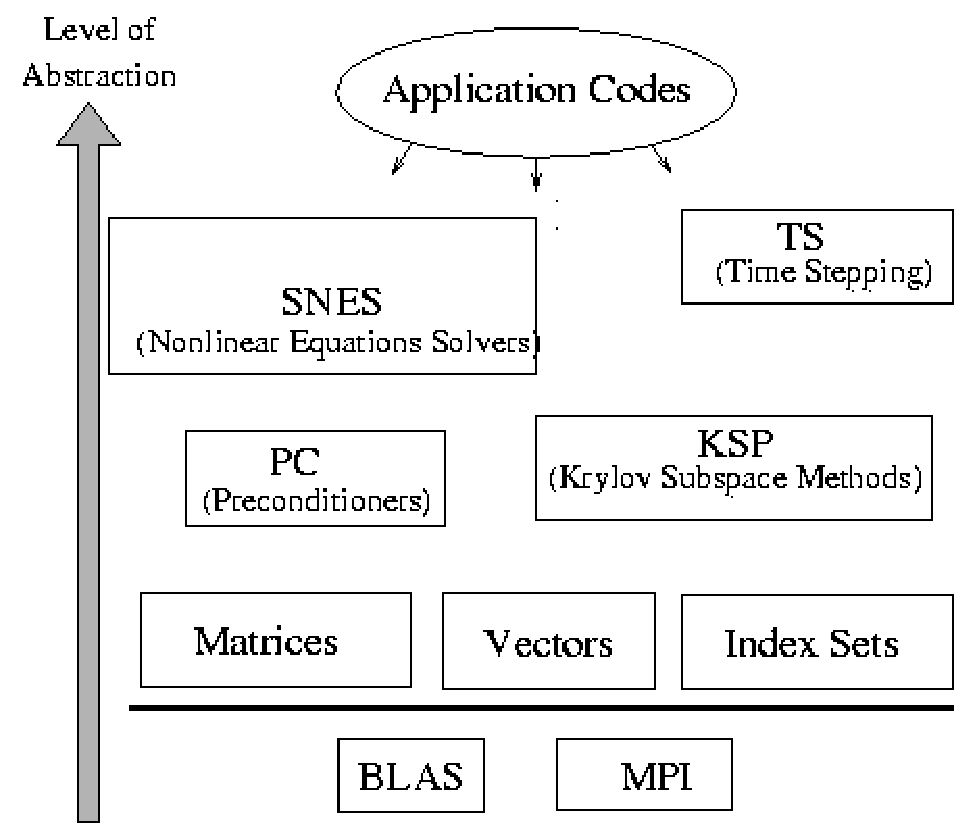
\includegraphics[width=8cm]{petscwww.eps}
\caption{\label{fig:petsc}Organization of the \petsc\ toolkit.}
\end{figure}

	\petsc\ components are discussed in detail in the users manual \citep{Balay:2002:PUM}. Each component manipulates a particular family of objects (for instance, vectors) and the operations one would like to perform on the objects. 
	The three basic abstract data objects are index sets, vectors and matrices. Built on top of this foundation are various classes of solver objects, which encapsulate virtually all information regarding the solution procedure for a particular class of problems, including the local state and various options such as convergence tolerances, etc. 
Some of the \petsc\ modules deal with 
\begin{itemize} 
\item index sets, including permutations, for indexing into vectors, renumbering, etc;
\item vectors;
\item matrices (generally sparse);
\item distributed arrays (useful for parallelizing regular grid-based problems);
\item Krylov subspace methods;
\item preconditioners, including multigrid and sparse direct solvers;
\item nonlinear solvers; and
\item timesteppers for solving time-dependent (nonlinear) PDEs.
\end{itemize}
Each of these components consists of an abstract interface (simply a set of calling sequences) and one or more implementations using particular data structures. \petsc\ is written in C, which lacks direct support for object-oriented programming. However, it is still possible to take advantage of the three basic principles of object-oriented programming to manage the complexity of such a large package. \petsc\ uses data encapsulation in both vector and matrix data objects. Application code access data through function calls. Also, all the operations are supported through polymorphism. The user calls a generic interface routine which then selects the underlying routine which handles the particular data structure. This is implemented by structures of function pointers. Finally, \petsc\ also uses inheritance in its design. All the objects are derived from an abstract base object. From this fundamental object, an abstract base object is defined for each \petsc\ object (\texttt{Mat}, \texttt{Vec} and so on) which in turn has a variety of instantiations that, for example, implement different matrix storage formats.

	\petsc\ provides clean and effective codes for the various phases of solving PDEs, with a uniform approach for each class of problems.  This design enables easy comparison and use of different algorithms (for example, to experiment with different Krylov subspace methods, preconditioners, or truncated Newton methods). Hence, \petsc\ provides a rich environment for modeling scientific applications as well as for rapid algorithm design and prototyping.

	Options can be specified by means of calls to subroutines in the source code and also as command-line arguments. Runtime options allow the user to test different tolerances, for example, without having to recompile the program. Also, since \petsc\ provides a uniform interface to all of its linear solvers ---the Conjugate Gradient, GMRES, etc. --- and a large family of preconditioners ---block Jacobi, overlapping additive Schwarz, etc. ---, one can compare several combinations of method and preconditioner by simply specifying them at execution time.
	
	The components enable easy customization and extension of both algorithms and implementations.  This approach promotes code reuse and flexibility, and separates the issues of parallelism from the choice of algorithms.  The \petsc\ infrastructure creates a foundation for building large-scale applications.
	Other advantages of \petsc\ are the following:
	\begin{itemize}
	\item High portability due to an elaborate Makefile system. Different architecture builds can coexist in the same installation. Where available, dynamic libraries are used to reduce disk space of executable files.
	\item Support for debugging and profiling: attachment to external debuggers, event logging, subroutine timing, convergence monitoring, etc. \petsc\ also has built-in graphics capabilities which allow for sparse pattern visualization, graphic convergence monitoring, operator's spectrum visualization and other user-defined operations.
	\item Programming interface for Fortran.
	\end{itemize}

%---------------------------------------------------
\chapter{Catalog of Solvers}
\label{cap:meth}

	This appendix provides a short description of all the eigenvalue solvers which are available in \slepc, including the interfaces to external libraries. In the case of ``native'' methods, that is, those methods that are implemented directly in \slepc, the description includes a sketch of the algorithm which is actually implemented.

	Table \ref{tab:defaults} summarizes the available native methods and shows the default values for some of their parameters.
\begin{table}[ht]
\centering
\begin{tabular}{cccc} \hline
Method   & \texttt{ncv} & \texttt{max\_it} & \texttt{tol} \\ \hline
\texttt{power}    &  1 & $\max(2000,100N)$ & $10^{-7}$ \\ 
\texttt{subspace} &  $\max(2\cdot nev,nev+8)$ & $\max(100,N)$ & $10^{-7}$ \\ 
\texttt{arnoldi}  &  $\max(2\cdot nev,nev+8)$ & $\max(100,N)$ & $10^{-7}$ \\ 
%\texttt{lanczos}  &  1 & $\max(2000,1000N)$ & $10^{-7}$ \\ 
\hline
\end{tabular}
\caption{\label{tab:defaults}Default parameter values for native algorithms available in \slepc.}
\end{table}


\section{\ident{power}}

This eigensolver covers several well-known single-vector iteration methods such as the Power Iteration, the Inverse Iteration and the Rayleigh Quotient Iteration.

When using the default spectral transformation (\ident{STSHIFT}), this solver provides an implementation of the Power Iteration. This is the simplest vector iteration method. It consists in premultiplying an initial vector by matrix $A$ repeatedly. Under certain conditions, the iteration converges to the dominant eigenvector (the one associated to the largest eigenvalue in magnitude). Then the approximate eigenvalue can be obtained by computing the Rayleigh quotient. Once an eigenvector has converged, deflation can be used to reveal the next ones. Note that this method will fail in the case that there is no unique dominant eigenvalue. Convergence can be very slow if separation of the dominant eigenvalue with the rest is small.

\begin{algorithm}[Basic Power Method\label{alg:pot}]~\rm
\begin{tabbing}
Input: Operator $O\!P$ and initial vector $v_0$\\
Output: Approximate dominant eigenpairs $(\theta,v)$ \\
xxxx\=xxx\=xxxxxxxxxxxxxxx\=\kill
\> Set $y=v_0$\\
\> For $k=1,2,\ldots$\\
\> \> Deflate previously converged eigenvectors \\
\> \> $v=y/\|y\|_B$ \\
\> \> $y=O\!Pv$ \\
\> \> $\theta=(y,v)_B$ \\
\> \> if $\|y-\theta v\|_2 < |\theta| \cdot \mathrm{tol}$, accept eigenpair \\
\> end
\end{tabbing}
\end{algorithm}
In the algorithm above, matrix $O\!P$ represents the operator, which can be any of the expressions in table \ref{tab:op}. Thus, the algorithm can be converted to the Inverse Iteration by simply specifying the \texttt{sinvert} transformation.

The Inverse Iteration works with a constant shift, that is, the operator is $(A-\sigma B)^{-1}B$ throughout the iteration. However, it is possible to change this behaviour by requesting the use of \emph{variable} shifts. There are two possibilities: Rayleigh shifts and Wilkinson shifts. This option can be changed with the command-line option \Verb!-eps_power_shift_type! or specified in the program source with the function \ident{EPSPowerSetShiftType}. 

The first alternative (\ident{rayleigh}) results in the well-known Rayleigh Quotient Iteration (RQI), where the new shift $\rho_k$ is computed as the Rayleigh quotient of the current approximate eigenvector $v$
\begin{equation}
\rho_k=R(v)=\frac{(Av,v)}{(Bv,v)}
\end{equation}
This strategy leads to cubic convergence. Note that changing the shift may imply refactorization of matrix $(A-\rho_k B)$.

The second alternative (\ident{wilkinson}) uses a more sophisticated formula for the shift \citep{Parlett:1998:SEP}.

%---------------------------------------------------
\section{\ident{subspace}}

The Subspace Iteration method is a generalization of the Power Method to $m$ initial vectors. Ortogonality of vectors is enforced in order to avoid linear dependence.

The implementation currently available in \slepc is based on SRRIT \citep{Bai:1997:ASF}. It performs a Rayleigh-Ritz projection procedure in order to improve convergence. Deflation is handled by locking converged eigenvectors. For better performance, orthogonalization and projection are performed only when necessary.

\begin{algorithm}[Subspace Iteration\label{alg:sub}]~\rm
\begin{tabbing}
Input: Operator $O\!P$ \\
Output: $m$ dominant Schur vectors $V$ and corresponding eigenvalues\\
xxxx\=xxx\=xxx\=xxxxxxxxxxxx\=\kill
\> Generate a set of initial orthonormal vectors $V\in\Co^{n\times m}$\\
\> For $k=1,2,\ldots$\\
\> \> Perform a Rayleigh-Ritz Projection step (algorithm \ref{alg:rrp})\\
\> \> Check convergence of eigenvalues \\
\> \> Orthogonalization loop \\
\> \> \> Repeatedly compute $V = O\!P\, V$ \\
\> \> \> Orthogonalize columns of $V$ \\
\> \> end \\
\> end
\end{tabbing}
\end{algorithm}

\begin{algorithm}[Rayleigh-Ritz Projection\label{alg:rrp}]~\rm
\begin{tabbing}
Input: Operator $O\!P$ and set of vectors $V$\\
Output: Schur vectors $V$ and quasi-triangular matrix $T$ \\
xxxx\=xxx\=xxxxxxxxxxxxxxx\=\kill
\> $T=V^H O\!P\, V$ \\
\> Reduce to Hessenberg form: $T=U_1^HTU_1$ \\
\> Reduce to quasi-triangular form: $T=U_2^HTU_2$ \\
\> $U=U_1U_2$ \\
\> $V=VU$ 
\end{tabbing}
\end{algorithm}

%---------------------------------------------------
\section{\ident{arnoldi}}

The version of the Arnoldi method implemented in \slepc uses locking and explicit restart. The orthogonalization technique can be chosen as described in chapter \ref{cap:eps}.

\begin{algorithm}[Arnoldi\label{alg:arn}]~\rm
\begin{tabbing}
Input: Matrix $A$, the initial vector $v_0$, and number of steps $k$ \\
Output: $(V_k,H_k,f_k)$ so that $AV_k=V_kH_k+f_ke_k^T$ \\
xxxx\=xxx\=xxx\=xxx\=xxxxxxxxxxxx\=\kill
\> Normalize $v_0$\\
\> Restart loop\\
\> \> For $j=1,2,\ldots,k$\\
\> \> \> $w=O\!Pv_j$ \\
\> \> \> For $i=1,2,\ldots,j$ \\
\> \> \> \> $h_{ij}=(w,v_i)$ \\
\> \> \> \> $w=w-h_{ij}v_i$ \\
\> \> \> end\\
\> \> \> $h_{j+1,j}=\|w\|_2\;$. \> \>If $h_{j+1,j}=0$ Stop \\
\> \> \> Reduce $H$ to (real) Schur form, $H=S\tilde{H}S^T$\\
\> \> \> $V=VS$ \\
\> \> end\\
\> \> Lock converged eigenpairs\\
\> \> Choose new initial vector\\
\> end\\
\end{tabbing}
\end{algorithm}

%---------------------------------------------------
%\section{\ident{lanczos}}
%
%\begin{algorithm}[Lanczos]~\rm
%\begin{tabbing}
%Input: Symmetric matrix $A$ and number of steps $k$ \\
%Output: $(V_k,T_k)$ being $\alpha_i$ and $\beta_i$ the diagonal and subdiagonal elements of $T_k$ \\
%xxxx\=xxx\=xxxxxxxxxxxxxxx\=\kill
%\> Choose a 1-norm vector $v_1$\\
%\> Initialize $\beta_1=0$, $v_0=0$\\
%\> For $j=1,2,\ldots,k$\\
%\> \> $w_j=Av_j-\beta_j v_{j-1}$ \\
%\> \> $\alpha_j=(w_j,v_j)$ \\
%\> \> $w_j=w_j-\alpha_j v_j$ \\
%\> \> $\beta_{j+1}=\|w_j\|_2$ \\
%\> \> $v_{j+1}=w_j/\beta_{j+1}$ \\
%\> end
%\end{tabbing}
%\end{algorithm}

%---------------------------------------------------
\section{Wrappers to External Libraries}
\label{sec:wrap}

	\slepc interfaces to several external libraries for the solution of eigenvalue problems. This section includes a short description of each of these packages as well as some hints for using them with \slepc.

	To use these eigensolvers, one needs to do the following.
	\begin{enumerate}
	\item Install the external software.
	\item Enable the utilization of the external software from \slepc by editing the file \Verb!${SLEPC_DIR}/bmake/${PETSC_ARCH}/packages!. For example, to use \arpack, one would specify the following variables with the appropriate paths:
	\begin{Verbatim}[fontsize=\small]
ARPACK_INCLUDE    = 
ARPACK_LIB        = -L/home/slepc/soft/ARPACK -lparpack -larpack
SLEPC_HAVE_ARPACK = -DSLEPC_HAVE_ARPACK
	\end{Verbatim}
	\item Build the \slepc libraries.
	\item Use the runtime option \Verb!-eps_type <type>! to select the solver.
	\end{enumerate}

	An exception to the above is \lapack, which should be already available in the \petsc{} installation.

	Table \ref{tab:defaults-ext} shows the default values for several parameters in each of the wrappers. Also, some of the interfaces can provide method-specific parameters.
\begin{table}[ht]
\centering
\begin{tabular}{ccccc} \hline
Method   &  \texttt{ncv} & \texttt{max\_it} & \texttt{tol} \\ \hline
\texttt{lapack}   &  - &         -          &    -      \\ 
\texttt{arpack}   &  $\max(20,2\!\cdot\!nev\!+\!\!1)$ & $\max(300,\lceil 2N/ncv\rceil)$ & $10^{-7}$ \\ 
\texttt{blzpack}  &  $\min(nev\!+\!\!10,2\!\cdot\!nev)$ & $\max(100,N)$ & $10^{-7}$ \\ 
\texttt{planso}   &  $nev$ & $\max(100,N)$ & $10^{-7}$ \\ 
\texttt{trlan}    &  $nev$ & $\max(100,N)$ & $10^{-7}$ \\ \hline
\end{tabular}
\caption{\label{tab:defaults-ext}Default values for wrappers to external
libraries.}
\end{table}

\section*{\underline{\lapack}}
	\begin{description}
	\item[References.]\citep{Anderson:1992:LUG}.
	\item[Website.] \url{http://www.netlib.org/LAPACK}.
	\item[Version.] 2.0 or later.
	\item[Summary.] \lapack\ (Linear Algebra PACKage) is a software package for the solution of many different dense linear algebra problems, including eigenvalue problems.

	\slepc explicitly creates the operator matrix in dense form and then the appropriate \lapack{} driver routine is invoked. Therefore, this interface should be used only for testing and validation purposes and not in a production code. The operator matrix is created by applying the operator to the columns of the identity matrix.

	Currently, only \lapack{} drivers for standard eigenvalue problems are
used. Generalized problems are transformed to standard ones.
	
	\item[Installation.]
	The \slepc interface to \lapack{} can be used directly.
	\end{description}

\section*{\underline{\arpack}}
	\begin{description}
	\item[References.]\citep{Lehoucq:1998:AUG}, \citep{Maschhoff:1996:PEP}.
	\item[Website.] \url{http://www.caam.rice.edu/software/ARPACK}.
	\item[Version.] Release 2 (plus patches).
	\item[Summary.] \arpack\ (ARnoldi PACKage) is a software package for the computation of a few eigenvalues and corresponding eigenvectors of a general $n\times n$ matrix $A$. It is most appropriate for large sparse or structured matrices, where structured means that a matrix-vector product $w \leftarrow Av$ requires order $n$ rather than the usual order $n^2$ floating point operations. 
	
	\arpack\ is based upon an algorithmic variant of the Arnoldi process called the Implicitly Restarted Arnoldi Method (IRAM). When the matrix $A$ is symmetric it reduces to a variant of the Lanczos process called the Implicitly Restarted Lanczos Method (IRLM). These variants may be viewed as a synthesis of the Arnoldi/Lanczos process with the Implicitly Shifted QR technique that is suitable for large scale problems. 

	It can be used for standard and generalized eigenvalue problems, both in real and complex arithmetic. It is implemented in Fortran 77 and it is based on the reverse communication interface. A parallel version, \parpack, is available with support for both MPI and BLACS.
	\item[Installation.]
	In order to use \arpack\ with \slepc, both the sequential version and the parallel version (\parpack) have to be installed. First, unbundle \texttt{arpack96.tar.gz}, then \texttt{parpack96.tar.gz}. Make sure you delete any \texttt{mpif.h} files that could exist in the directory tree. Also it is recommended to unpack the patch files \texttt{patch.tar.gz} and \texttt{ppatch.tar.gz}. After that, modify the \texttt{ARmake.inc} file and then compile the software with \texttt{make all}.
	\end{description}

\section*{\underline{\blzpack}}
	\begin{description}
	\item[References.]\citep{Marques:1995:BDU}.
	\item[Website.] \url{http://www.nersc.gov/\~{}osni/\#Software}.
	\item[Version.] 04/00.
	\item[Summary.] \blzpack\ (Block LancZos PACKage) is a standard Fortran 77 implementation of the block Lanczos algorithm intended for the solution of the standard eigenvalue problem $Ax=\mu x$ or the generalized eigenvalue problem $Ax=\mu Bx$, where A and B are real, sparse symmetric matrices. The development of this eigensolver was motivated by the need to solve large, sparse, generalized problems from free vibration analysis in structural engineering. Several upgrades were performed afterwards aiming at the solution of eigenvalue problems from a wider range of applications.

	\blzpack\ uses a combination of partial and selective re-orthogonalization strategies. It can be run in either sequential or parallel mode, by means of MPI or PVM interfaces, and it uses the reverse communication strategy.
	\item[Installation.] For the compilation of the \texttt{libblzpack.a} library, first check the appropriate architecture file in the directory \texttt{sys/MACROS} and then type \texttt{creator -mpi}.
	\item[Specific options.] The \slepc interface to this package allows
to specify the block size with the function \ident{EPSBlzpackSetBlockSize} or
at run time with the option \Verb!-eps_blzpack_block_size <size>!.

	For the spectrum slicing feature, \slepc allows the programmer to provide the computational interval with the option \Verb!-eps_blzpack_interval!, or with the function \ident{EPSBlzpackSetInterval} in the program source. Also, the function \ident{EPSBlzpackSetMatGetInertia} can be used to provide a function for computing the intertia of the matrix.
	\end{description}

\section*{\underline{\planso}}
	\begin{description}
	\item[References.]\citep{Wu:1997:PLM}.
	\item[Website.] \url{http://www.nersc.gov/research/SIMON/planso.html}.
	\item[Version.] 1.0 (07/1997).
	\item[Summary.] This package implements the Lanczos algorithm with partial re-orthogonalization for symmetric generalized eigenvalue problems. It is based on the sequential package \lanso\ maintained by B. Parlett. \planso\ is implemented in Fortran 77 using MPI and the user must provide functions for matrix-vector products.

The current version uses the Omega-recurrence to simulate the loss of orthogonality among the Lanczos vectors and maintains semiorthogonality.  This is sufficient to guarantee that eigenvalues are computed accurately, but under extreme conditions the eigenvectors may not be as accurate as the eigenvalues.
	\item[Installation.] Change \texttt{Make.inc} in the top level directory to set appropriate compiler and flags to use. Then type \texttt{make lib plib}.
	\end{description}

\section*{\underline{\trlan}}
	\begin{description}
	\item[References.]\citep{Wu:2001:TLM}.
	\item[Website.] \url{http://www.nersc.gov/\~{}kewu/trlan.html}.
	\item[Version.] 1.0 (03/1999).
	\item[Summary.] This package provides a Fortran 90 implementation of the dynamic thick-restart Lanczos algorithm. This is a specialized version of Lanczos that targets only the case in which one wants both eigenvalues and eigenvectors of a large real symmetric eigenvalue problem that cannot use the shift-and-invert scheme. In this case the standard non-restarted Lanczos algorithm requires to store a large number of Lanczos vectors which can cause storage problems and make each iteration of the method very expensive.

	\trlan{} requires the user to provide a matrix-vector multiplication routine. The parallel version uses MPI as the message passing layer. 
	\item[Installation.] To install this package, it is necessary to have access to a Fortran 90 compiler. The compiler name and the options used are specified in the file called \texttt{Make.inc}. To generate the library, type \texttt{make libtrlan\_mpi.a} in the \texttt{TRLan} directory.
	\end{description}

